\section{Fila de espera no Sistema Único de Saúde}
    O Sistema Único de Saúde (SUS) é um dos maiores sistemas públicos de saúde do mundo, sendo o único a
    garantir assistência integral e completamente gratuita para a totalidade da população \citeonline{SOUZA2002}. Diferentemente de outros países, no Brasil, mesmo quem opta por um plano de saúde privado tem o direito de ser atendido em qualquer unidade do Sistema Único de Saúde.
   
   \subsection{Financiamento do SUS}
   
     O financiamento do SUS é uma responsabilidade comum entre o governo nacional, estadual e municipal que realizam a destinação de porcentagens diferentes de seu orçamento para o SUS, dividia da seguinte forma \citeonline{CONASS}:
    \begin{itemize}
        \item União: A Emenda Constitucional n. 86 de 17 de março de 2015 definiu que a partir de 2016 a União aplicará, anualmente, em ações e serviços públicos de saúde, o montante correspondente ao valor da Receita Corrente Líquida (RCL) do respectivo exercício financeiro, não podendo ser inferior a 15\%, mas que será cumprido progressivamente
        \item  Estados e Distrito Federal: No mínimo 12\% da arrecadação dos impostos são destinadas a ações e serviços públicos de saúde, sendo deduzidas as parcelas que forem transferidas aos municípios;
        \item Municípios e o Distrito Federal: Anualmente aplicam em ações e serviços públicos de saúde, no mínimo, 15\% da arrecadação dos impostos.
    \end{itemize} 

   
   	\subsection{Funcionamento do SUS}
   	
    O Governo Federal tem o dever de fiscalizar e elaborar mecanismos de apoio para que  estados e municípios possam oferecer serviços de saúde.

   É na instância municipal que o paciente dá a entrada no sistema, por meio da UBS (Unidade Básica de Saúde) ou pela equipe da Unidade Saúde da Família (USF) que são profissionais que acompanham um número de famílias em uma determinada área geográfica. Na UBS é realizado o atendimento com hora marcada e deve sempre haver médicos de três especialidades: clínico geral, pediatra e ginecologista. Nestas unidades é oferecido um primeiro atendimento, afim de realizar uma triagem e quando necessário solicitar o encaminhamento para as demais especialidades \citeonline{CONTE2017}.
   
   Na imagem XX abaixo, é apresentado o fluxo pelo qual o paciente é submetido dentro do SUS desde o primeiro contato até um atendimento especializado ou internação:
    
     \begin{figure}[htbp]
        	\centering
            \caption{Funcionamento SUS}
            \label{fig:images/fluxograma-trajetoria-usf-pe}
            
\includegraphics[width=0.9\linewidth]{images/funcionamento-sus.png}
            \fdireta{SECRETARIAMG}
        \end{figure}
    
    Ainda na UBS, caso o paciente necessite de um atendimento emergencial, a UPA (Unidade de Pronto Atendimento) é quem o recebe. As UPAs são unidades de complexidade intermediária entre  as UBSs e a emergência dos hospitais, portanto, servem para "desafogar" as filas dos hospitais. Segundo o Ministério da Saúde, 97\% dos casos que chegam as UPAs são solucionados \citeonline{BRASIL2012}. Os pacientes que procuram as UPAs são avaliados de acordo com a classificação de risco, ou seja, os casos mais graves terão prioridade.
    
     \subsection{Filas de espera}
    
    O caminho que um paciente percorre até o efetivo atendimento pode ser longo e muitas vezes acaba precisando retornar no início do fluxo de atendimento. O trabalho de \citeonline{SOUZA2014}, avaliou as condições de acesso integral dos usuários a partir do caminho percorrido desde a atenção básica até a especializada na rede assistencial de Recife - PE. O fluxograma do caminho percorrido pelos pacientes é exibido na figura XX:
    
     \begin{figure}[htbp]
        	\centering
            \caption{Fluxograma Descritor do acesso do usuário da atenção primária à atenção especializada.}
            \label{fig:images/fluxograma-trajetoria-usf-pe}
            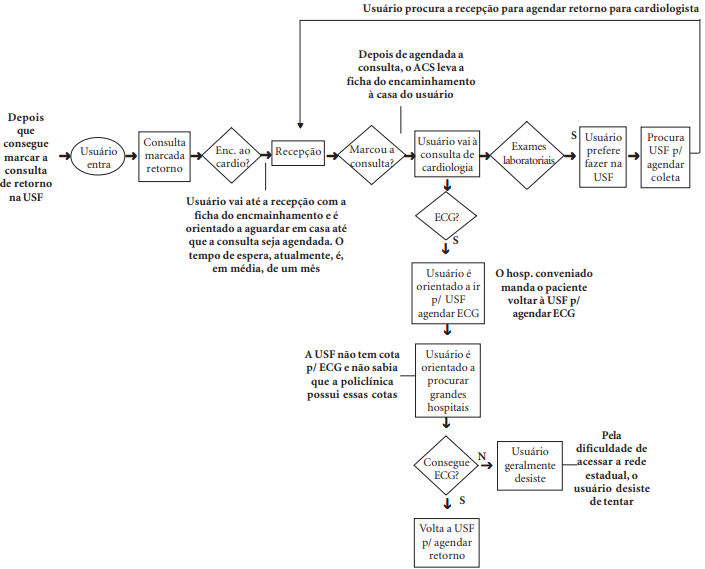
\includegraphics[width=0.8\linewidth]{images/fluxograma-trajetoria-usf-pe}
            \fdireta{SOUZA2014}
        \end{figure}
        
    Quando um médico de família encaminha um usuário ao especialista, este procura a recepção da USF para entregar a sua ficha de encaminhamento ao profissional responsável pela marcação das consultas que por sua vez faz o contato telefônico com a Central de Regulação do Recife para o agendamento.
    A demora no agendamento das consultas especializadas é uma das barreiras de acesso para o atendimento integral da população. No estudo, ainda é citado que a inexistência de critérios definidos para a escolha do serviço de referência no qual os usuários serão agendados é outro aspecto desordenador do acesso, essa definição cabe ao pessoal administrativo, ou os ‘marcadores das consultas’. Outro aspecto que chama a atenção, como
    elemento desordenador, é o fato de o agendamento das consultas ser realizado, predominantemente, pela ordem de chegada das fichas de encaminhamento na recepção. Com exceção dos casos em que o próprio médico sinaliza a ‘urgência’ ou ‘prioridade’ dos pacientes, é o responsável pela marcação das consultas que tenta priorizar
    quem deverá ter acesso e agendamento prioritário. Esse aspecto demonstra que a análise de risco clínico não se coloca como atividade consolidada no processo de trabalho das equipes de saúde da família \citeonline{SOUZA2014}.
    
    Um outro problema abordado na literatura quando se trata de atendimento especializado, é a questão do absenteísmo. No trabalho de \cite{URSULA2018} é realizada uma análise do impacto da fila da espera no absenteísmo de exames e consultas. O estudo revela que as maiores
    probabilidades de ocorrência de absenteísmo são obtidas de modo geral em
    procedimentos que ultrapassam os 60 dias de espera. O trabalho concretiza que a redução do tempo de espera para menos de 60 dias possibilitou a diminuição significativa do absenteísmo, o que repercute na diminuição do agravamento de doenças e nos custos ao sistema de saúde. 
    
    A fila de espera não é um entrave apenas no SUS, é um problema em cerca da metade dos países da OECD \cite{SICILIANI2004}. Recursos financeiros escaços, quantidade de vagas, gestão e estrutura são também presentes em outros países, como o Sistema Nacional de Saúde espanhol (SNS). No trabalho de Conill (2011), para o enfrentamento destas barreiras no acesso ao sistema de saúde, foram realizadas iniciativas que a proporcionassem a continuidade assistencial. Foi adotada a medida de circuitos preferenciais. Essa estratégia serve para encaminhar da atenção primária com preferência os usuários com suspeitas de alguma etiologia específica. Uma parceria entre o Fórum Espanhol de Pacientes em conjunto com a Universidade de Harvard (EUA), desenvolveu uma pesquisa com 3.010 cidadãos, para avaliar a confiança dos espanhóis no sistema nacional de saúde. Entre outros aspectos, este trabalho revelou que, sem distinção de classe social, área geográfica ou densidade demográfica, as listas de espera são o principal problema dos serviços de saúde espanhóis para 78\% dos entrevistados. \citeonline{LOPEZ2007} 
    Vale salientar que as filas de espera do atendimento básico para o especializado, não são as únicas onde o paciente encontra problemas, filas como de urgências e cirurgias também são dificuldades reais no SUS. O trabalho de \citeonline{KRISHNAMURTI2005}, trás uma abordagem das filas de espera para cirurgias otorrinolaringológicas no SUS. O trabalho descreve que o maior afunilamento acontece na obtenção da consulta no ambulatório de otorrinolaringologia, ou seja no atendimento especializado (seta nº 3, na figura XX).
    
    \begin{figure}[htbp]
        	\centering
            \caption{As setas tracejadas representam os pontos críticos no processo de obtenção do tratamento.}
            \label{fig:images/fluxo-fila-cirurgia-otorrino}
            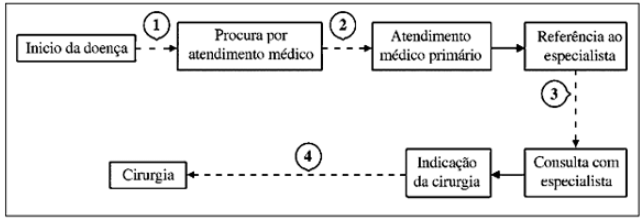
\includegraphics[width=0.9\linewidth]{images/fluxo-fila-cirurgia-otorrino.png}
            \fdireta{KRISHNAMURTI2005}
        \end{figure}
        
    O trabalho ainda discute um tema importante, ao questionar se os indivíduos destas filas de espera realmente passaram por vias regulares e justas para o atendimento. Muitos que tem a possibilidade, procuram outras formas de se obter a consulta, surgem então os pedidos de "consulta extras". São os chamados "PAFs" ou "PAFUNCIOs" tão conhecidos do médico que trabalha em serviço público: "Parente ou Amigo de Funcionário".

    No artigo, o autor relata que ocorre uma pressão não só diretamente sobre os médicos, mas também sobre enfermeiros, auxiliares de enfermagem e demais funcionários. Os funcionários responsáveis pela marcação das consultas também são pressionados, de modo que é preciso atentar para o fato de que mesmo o paciente que parece ter tido a sua consulta marcada por vias regulares pode ter sido beneficiado nessa marcação. Mais grave, já há casos (crimes, melhor dizendo) de pessoas e funcionários que vendem estas consultas ou mesmo um lugar na fila da triagem do hospital. O médico, sem saber, passa a ser o instrumento de um lucrativo negócio: o do agenciamento da medicina pública \citeonline{KRISHNAMURTI2005}.
    Estes pacientes, independente da gravidade de suas queixas e do seu direito inquestionável ao atendimento, estão na realidade "furando" uma fila virtual de espera. Pode-se chegar a extremos em que o número de pessoas "furando" a fila é tal a ponto de criar uma fila paralela, com fluxo contínuo, enquanto a fila principal e legítima permanece quase parada. Concluindo, o trabalho ainda deixa claro que é necessário o enfrentamento da questão, e que os pacientes devem ser informados sobre sua condição, de preferência por escrito, da indicação cirúrgica, da existência da fila, dos critérios de prioridade nesta fila, da quantidade de pessoas à sua frente e de uma estimativa do tempo até sua cirurgia, deixando-se claro tratar-se apenas de uma estimativa.
    
    --TOPICO DESENVOLVIMENTO
    
    SUBTOPICO DE DESENVOLVIMENTO, Critérios para priorização doa tendimento:
    
    Entende-se por prioridade no atendimento cirúrgico a própria ordem em que estes pacientes serão atendidos, isto é, submetidos à cirurgia. Até então consideramos o tempo de espera na fila como o principal critério de prioridade. Entretanto, este não é obviamente o único critério que deve ser considerado. Pacientes que necessitam de cirurgias de emergência (uma mastoidite aguda ou uma sinusite com complicação intra-orbitária) são exemplos extremos em que a prioridade independe do tempo de espera.

Da mesma forma, mesmo em cirurgias eletivas, a prioridade na realização da cirurgia deve também levar em conta a gravidade e urgência de cada caso. Pacientes com casos mais graves devem ser operados antes daqueles com casos menos graves, independente do tempo de acompanhamento no serviço. É preciso, todavia, que estes critérios de prioridade sejam claros e bem estabelecidos para um bom funcionamento do serviço.

Por gravidade, entenda-se o grau de sofrimento, limitações ou risco de vida que a doença impõe ao paciente. O conceito de urgência leva em conta a gravidade aliada aos possíveis benefícios da cirurgia em relação à história natural da doença, além de fatores sociais e filosóficos7. Um paciente com câncer de laringe em estado inicial, por exemplo, não é um caso grave no momento, uma vez que só apresenta disfonia leve, mas é um caso urgente pois a cirurgia tem grande impacto na evolução da doença. Por outro lado, um paciente em estado terminal é sem dúvida um paciente grave, mas não urgente pois a cirurgia tem menor impacto na história natural de sua doença. É com base nestes conceitos que cada serviço deve estabelecer seus critérios de prioridade para cada cirurgia.

Em linhas gerais, alguns critérios devem ser destacados:

1. História de complicações

a. Complicações sistêmicas. 
b. Complicações em órgãos e estruturas adjacentes. 
c. Complicações locais.

1. Pacientes com comorbidades graves. 
2. Pacientes com sinais clínicos ou radiológicos de doença avançada. 
3. Menores de idade e idosos. 
4. Fatores sócio-econômicos.

O histórico de complicações infecciosas ou de outra natureza é talvez o critério de prioridade mais importante, pois representa um risco aumentado de óbito. As complicações devem ser estratificadas em seus graus de severidade e possibilidade de recorrência. Como regra geral, as complicações infecciosas intra-cranianas (meningite, abscesso intra-craniano, empiema) são consideradas mais graves, pelo risco de vida e alta taxa de recorrência. Em seguida vêm as complicações em órgãos adjacentes (como as orbitárias na polipose nasal) e restritas ao órgão alvo da doença (como a paralisia facial no colesteatoma).

Os pacientes com comorbidades graves são outro grupo prioritário. Entenda-se por comorbidade outras afecções sistêmicas com ou sem relação com a doença otorrinolaringológica e que a revestem de maior gravidade ou possibilidade de complicação pela interação mútua das duas condições. Exemplos clássicos são a associação entre polipose e asma ou entre hipertrofia adenoamigdaliana e síndrome de apnéia obstrutiva do sono. Entretanto, outras afecções sistêmicas, mesmo sem relação direta com a doença otorrinolaringológica, devem ser levadas em conta, tais como insuficiência renal, transplantados (ou candidatos a transplante), pacientes com SIDA, diabéticos graves, etc.

Pacientes com sinais clínicos ou radiológicos de doença avançada que sugiram a possibilidade aumentada de evolução para complicações também devem ser priorizados. Colesteatomas com erosão avançada do tegmen timpani encaixam-se neste grupo.

Pelo estatuto da criança e do adolescente8 e pelo estatuto do idoso9, ambos já em vigor em nosso país, estes grupos etários devem sempre ser priorizados no atendimento em qualquer hospital público e na implantação de qualquer política de saúde. Portanto, também devem ser considerados casos prioritários.

Já os fatores sócio-econômicos são sem dúvida importantes, mas a sua consideração no estabelecimento dos critérios de prioridade é bastante controversa. Alguns serviços, por exemplo, priorizam a cirurgia de pacientes que moram em municípios distantes ou mesmo em outros estados, por entenderem que o acompanhamento prolongado em hospital tão distante de suas residências causa transtorno e sofrimento maiores. Outros podem considerar relevantes questões mais sutis, como o impacto da doença na vida profissional do paciente, ou o caso de pacientes que cuidam de parentes doentes e que portanto não têm tempo para cuidar de sua própria saúde, etc. As possibilidades são infinitas. Por isso é necessário que haja abertura para ampla discussão dos critérios a serem estabelecidos e também para casos particulares. O uso do livre entendimento e do bom senso da equipe cirúrgica não pode ser negligenciado, desde que se aplique sempre os mesmos critérios para todos os casos.
(http://www.scielo.br/scielo.php?script=sci_arttext&pid=S0034-72992005000300001)
    

--citar conil e ver se el falar isso mesmo
Além desses casos, no aspecto de organização, a fila de espera pode adotar
na prática outros recursos de ordenamento. Sarmento Júnior, Tomita e Kos. (2014)
abordam o recurso da fila do “esperar para ver” (“wait and see list”), como uma boa
alternativa para gerenciar os casos etiológicos que podem ser “tratados” durante o
tempo de espera. Esses casos são monitorados e transferidos de fila. Um exemplo
apontado pelos autores são os casos de cirurgias oftalmológicas. Cria-se uma fila
para os casos que a indicação para cirurgia ainda não é exata, fazendo então o
acompanhamento desses pacientes, para um futuro encaminhamento para a fila
conforme o retrocesso ou avanço de uma patologia.
Contudo, a literatura apresentou os dados estatísticos das taxas crescentes
do impacto da fila de espera e a importância de implantar ferramentas que auxiliem
no processo de otimização dos serviços de saúde, nesse caso, voltado para os
fatores que interferem na fila de espera e nas perdas causadas pelo absenteísmo.
Ou seja, adotar alternativas para diminuir esse problema no sistema de saúde e
buscar atender as necessidades do município com relação à oferta de serviços
especializados (ALBIERI, 2015).
Em nível nacional faz-se necessário incremento na estratégia de regulação,
que fomenta a efetivação do ordenamento do de acesso aos serviços de saúde
    
    -colocar na instrocução o conteudo abaixo
    
    Como o número de pacientes que necessitam de um atendimento especializado é maior que a quantidade de vagas oferecidas, uma fila de espera é criada. A fila de espera é uma lista de pacientes que necessitam de um mesmo tratamento ou serviço médico cuja demanda é maior que a oferta.\citeonline{KRISHNAMURTI2005} As
    especialidades médicas e os serviços de exames possuem uma capacidade limitada de atendimentos, isto é, um número finito de vagas.
    
    Longos tempos de espera têm se constituído em um problema comum em diferentes sistemas públicos de saúde. Além de um importante determinante da satisfação dos profissionais e usuários, o tempo de espera é um indicador da qualidade dos serviços, por estar relacionado à capacidade de resposta do sistema às necessidades de atenção à saúde da população. \citeonline{Gazzinelli2014} No Brasil, o longo tempo de espera para consultas especializadas está entre as principais barreiras ao acesso a cuidados integrais à saúde no Sistema Único de Saúde (SUS).
    
    Não há controle das listas de espera ou uma estratégia padrão para organizá-las. Ficando a critério das instituições a escolha da forma que sistematizará, se por especialidade, prestador ou por data, gerando então diversas filas e informações que dificultam inclusive o monitoramento e gerenciamento das mesmas \citeonline{URSULA2018}.
    
    Como cada município pode fazer a gestão da fila, nem sempre é um especialista que elabora a fila de espera, podendo ainda não utilizar critérios corretos para a ordem de atendimento. Algumas possíveis soluções para o problema da fila de espera merecem discussão. Medidas que aumentem a oferta de serviços especializados estão, frequentemente, entre as principais estratégias para a redução do tempo de espera. Mas entende-se que simplesmente aumentar a oferta de consultas, visando reduzir a lista de espera, apenas encorajaria o número de encaminhamentos. A solução passa também, provavelmente, por melhor comunicação entre o médico clínico geral, ou médico de comunidades, e o especialista. Para isso, é necessária estruturação adequada e consistente dos serviços de atenção primária, com melhorias nos sistemas de agendamento e de encaminhamento.\citeonline{Gazzinelli2014}
    
  